\chapter{Domain modeling process}

In our thesis, we consider a domain modeling process stating with a domain description $T$ acquired from stakeholders and knowledge sources such as internal documentation, manuals, or state law. $T$ can be a well-curated text, but may also encompass varied interpretations articulated by different stakeholders at various levels of detail. A modeling expert translates $T$ into a domain model $M$ in a sequence of steps.

A domain model $M = (\mathcal{C}, \mathcal{P})$ consists of a set of classes $\mathcal{C}$ and properties $\mathcal{P}$.

A class $C \in \mathcal{C}$ has its $name(C)$ which identifies $C$ in $M$ and briefly characterizes the semantics of $C$. The class $C$ also has a $description(C)$ that describes the semantics of $C$.

A Property $P \in \mathcal{P}$ has also $name(P)$ and $description(P)$ used for the same purposes. It has a $cardinality(P)$ that refers to the specification of the number of instances of one domain element that can or must be associated with each instance of some class. It also has a source class, such that $source(P) \in \mathcal{C}$ and it can have a target class such that $target(P) \in \mathcal{C}$. $P$ is a binary association if $target(P)$ is defined otherwise, $P$ is an attribute. If $P$ is an attribute then it also has $dataType(P)$ which defines the data type of $P$.

These basic modeling constructs are prevalent in real conceptual models \cite{Keet2015}, so their automation could have a significant impact. We distinguish the following steps.


\section{Steps}
\label{modeling_steps}
\begin{description}
\item [Design a class] For a concept in $T$, create a class $C$ with a designated $name(C)$.

\item[Design an attribute for a class] For a class $C$ and a concept in $T$ that characterizes $C$, create an attribute $P$, where $C = source(P)$, and define its $name(P)$.

\item[Design an association for a class] For a class $C$ and a concept in $T$ that describes a relationship of $C$ with another concept, create an association $P$ such that $C = source(P)$ or $C = target(P)$, and define its $name(P)$. If not yet represented, create a class $D$ for the other concept and specify its $name(D)$.

\item [Design a description for a class] For a class $C$ and a concept in $T$ that characterizes $C$, define $description(C)$.

\item [Design a description for an attribute] For an attribute $P$ and a concept in $T$ that characterizes $P$, define $description(P)$.

\item [Design a description for an association] For an association $P$ and a concept in $T$ that characterizes $P$, define $description(P)$.

\item [Design a data type for an attribute] For an attribute $P$ and a concept in $T$ that characterizes $P$, define $dataType(P)$.

\item [Design a cardinality for an attribute] For an attribute $P$ and a concept in $T$ that characterizes $P$, define $cardinality(P)$.

\item [Design a cardinality for an association] For an association $P$ and a concept in $T$ that characterizes $P$, define $cardinality(P)$.
\end{description}


\section{Example}

Consider the following domain description $T$: ``In this company, every employee works in some department. Each employee is uniquely identified by his ID.'' Figure \ref{fig:simple-employee-domain-model} shows how a corresponding domain model can look like. It contains a class \textit{employee} with the attribute \textit{ID} and the association \textit{works in} between the classes \textit{employee} and \textit{department}.

\begin{figure}[!h]
    \centering
    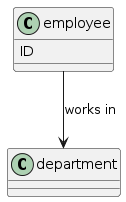
\includegraphics[scale=0.65]{img/domain-modeling-steps-example.png}
    \caption{\centering Simple domain model example}
    \label{fig:simple-employee-domain-model}
\end{figure}

To create the described domain model when starting from an empty domain model the following steps can be executed:

\begin{enumerate}
\item design a class: for the concept ``In this company, every employee works in some department'' create a class $C$ such that \textit{employee} = $name(C)$
\item design a class: for the concept ``every employee works in some department'' create a class $C$ such that \textit{department} = $name(C)$
\item design an attribute: for the class \textit{employee} and the concept ``Each employee is uniquely identified by his ID'' create the attribute $P$ such that \textit{ID} = $name(P)$ and \textit{employee} = $source(P)$
\item design an association: for a class \textit{employee} and the concept ``every employee works in some department'' create the association $P$ such that \textit{works in} = $name(P)$, \textit{employee} = $source(P)$ and \textit{department} = $target(P)$
\end{enumerate}

For providing more information for this domain model, the other mentioned steps can be used for defining descriptions of the modeled elements, for defining data types of the modeled attributes and for defining cardinalities of the modeled attributes and associations.